% !TEX root = vorlage.tex

\pagenumbering{arabic}
\ohead{\headmark}
\section{Einleitung}\label{section:introduction}
\subsection{Continental}\label{section:continental}
Die Continental AG ist ein weltweit tätiger deutscher Automobilzulieferer mit Hauptsitz in Hannover. Zur Zeit werden circa 230.000 Mitarbeiter weltweit beschäftigt, welche an über 400 Standorten in insgesamt 61 Ländern tätig sind.\\

Continental ist in fünf \acl{BA}s aufgeteilt mit diversen \acl{BU}s pro \acl{BA}.
Wetzlar gehört Zentral zur \acl{BA} \acl{VNI} und beherbergt alle drei in Abbildung \ref{fig:5business_areas} aufgelisteten \acl{BU}s.\\

Der Standort wurde 1955 von Philips gegründet und 2007 von Continental übernommen.
Zur Zeit fokussiert sich das Produkt Portfolio von Wetzlar auf die Entwicklung von digitalen Kombiinstrumenten, sowie \acl{TCU}s.\\

\begin{figure}[!h]
	\centering	
	\fbox{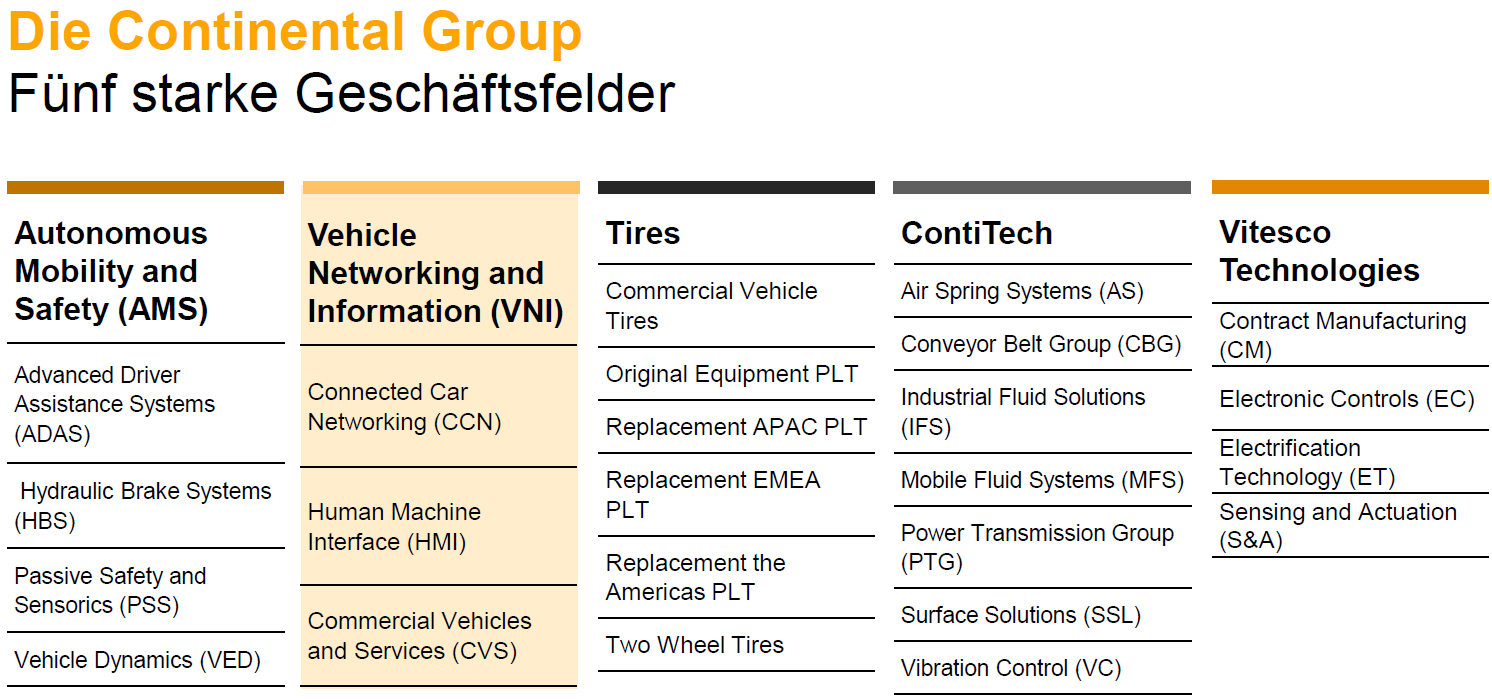
\includegraphics[width=1\textwidth]{Bilder/struktur.png}}
	\caption{5 Business Areas von Continental}
	\label{fig:5business_areas}
\end{figure}


\subsection{Abteilung Persistence}\label{section:persistence}

Das Persistence Team gehört zur \acl{BU} \acl{CE}.
Dabei sind sie Teil des Softwareplatform Projekts \acl{IIP}, welches sich mit der Entwicklung einer high performance Softwareplatform
für diverse Varianten beschäftigt.
Hierbei liegt der Fokus auf der Wiederverwendbarkeit der Architektur, sowie der Platform für verschiedene Kunden.

Hierbei kümmert sich das Team um den Zugriff auf den Speicher der Hardware, sowie um die Zuteilung der Speicherpartitionen.


\subsection{Problemstellung}\label{section:problemstellung_und_ziel}

Für zukünftige Anwendungsfälle sollen einige der \acl{IIP} Varianten ein kleines Filesystem bekommen,
mit welchem einfache Daten von den Applikationen gespeichert werden können.
Allerdings kostet das mit Integrity OS mitgelieferte Filesystem pro produziertem hardware target Geld.
Da dieses außerdem noch die benötigten Funktionen übertrifft, soll nach einer kostengünstigen Alternative gesucht werden.\\


\subsection{Proof of Concept}
Das \acl{PoC} kommt ursprünglich aus dem Projektmanagement und wird genutzt um die Durchführbarkeit eines Vorhabens zu belegen.
Dabei kommt es entweder zu einem positiven oder negativen Ergebnis, welche die weitere Projektplanung bestimmt.\\

Meistens wird bei dem \acl{PoC} auch ein Prototyp entwickelt, welcher die Kernfunktionalitäten des Vorhabens aufweist.
Gerade bei software orientierten Projekten ist der Prototyp notwendig um Schnittstellen um die Umgebung zu identifizieren.\\

Mit Hilfe des \acl{PoC} können außerdem Risiken und Entscheidungen für den weiteren Projektverlauf minimiert werden.
Zum einen werden fürh kritische Anforderungen an die Anwendung validiert, zum Anderen wird das Risiko, sowie das Budget durch den Prototypen minimiert.\\


\subsection{Motivation}
Mit einer eigenen Implementierung eines Filesystems kann Geld für die spätere Produktion gespart werden,
was je nach Menge der produzierten Steuergeräte eine hohe Summe an Geld sparen kann.
Außerdem ist die Software, welche während der \acl{PoC} entsteht später in jedem Gerät welches produziert wird vertreten.\\


\subsection{Ziel}
Ziel des Projektstudiums ist es ein \acl{PoC} für die Implementierung eines Filesystems zu erstellen und
die darauffolgende Implementierung des selbigen im \acl{IIP} Projekt.